\documentclass{beamer}
\usepackage{tikz}
\usetikzlibrary{positioning}

\tikzset{onslide/.code args={<#1>#2}{%
  \only<#1>{\pgfkeysalso{#2}} % \pgfkeysalso doesn't change the path
}}
\tikzset{temporal/.code args={<#1>#2#3#4}{%
  \temporal<#1>{\pgfkeysalso{#2}}{\pgfkeysalso{#3}}{\pgfkeysalso{#4}} % \pgfkeysalso doesn't change the path
}}

\tikzstyle{highlight}=[red,ultra thick]


\begin{document}
\begin{frame}
 \begin{figure}[h]
  \begin{centering}
  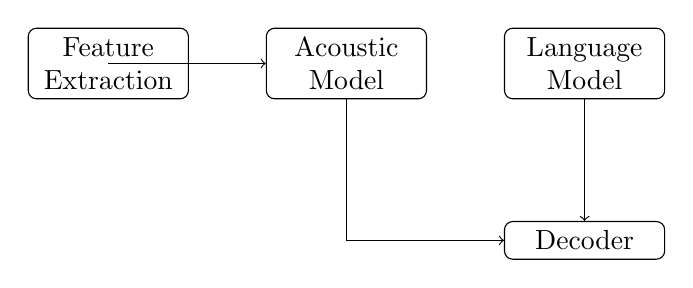
\begin{tikzpicture}[
  	system/.style={draw,rectangle,rounded corners=3,minimum width=2cm,text width=1.8cm,text centered},
  	node distance=2cm
  ]
    \node [system,onslide=<3->{highlight},anchor=center] (fe) {Feature Extraction};
    \node [system,onslide={<2,4>{green}}] (am) [right=of fe.center] {Acoustic Model};
    \node [system,temporal=<3>{blue}{highlight}{green}] (lm) [right=of am.center] {Language Model};
    \node [system] (d) [below=of lm.center] {Decoder};

    \draw[->] (fe) |- (am);
    \draw[->] (am) |- (d);
    \draw[->] (lm) -- (d.north);

  \end{tikzpicture}
  \end{centering}
  \end{figure}
\end{frame}
\end{document}
